\documentclass[english]{article}
\usepackage[italian]{babel} 
\usepackage[T1]{fontenc}
\usepackage[utf8x]{inputenc}
\usepackage{float}
\usepackage{graphicx}
\makeatletter
\usepackage[a4paper,top=2cm,bottom=2cm,left=2cm,right=2cm]{geometry}
\usepackage{enumitem}
\usepackage{subfig}
\usepackage{amsthm}
\usepackage{amsmath}
\usepackage{epstopdf}
\usepackage{fancyhdr}
\usepackage{booktabs,array}
\newcommand*{\eacc}{\MakeUppercase{è }}

% Pacchetto per la gestione del testo colorato
\usepackage{color}

% Pacchetto che permette l'inserimento di codice Matlab formattato
\usepackage{listings} % inserisce listati di programmi
\definecolor{commenti}{rgb}{0.13,0.55,0.13}
\definecolor{stringhe}{rgb}{0.63,0.125,0.94}
\lstloadlanguages{Matlab}
\lstset{% general command to set parameter(s)
framexleftmargin=4mm,
frame=single,
keywordstyle = \color{blue},% blue keywords
identifierstyle =, % nothing happens
commentstyle = \color{commenti}, % comments
stringstyle = \ttfamily \color{stringhe}, % typewriter type for strings
showstringspaces = false, % no special string spaces
emph = {for, if, then, else, end},
emphstyle = \color{blue},
firstnumber = 1, % numero della prima linea
numbers =left, %  show number_line
numberstyle = \tiny, % style of number_line
stepnumber = 5, % one number_line after stepnumber
numbersep = 5pt,
language = {Matlab}, % per riconoscere la sintassi matlab
extendedchars = true, % per abilitare caratteri particolari
breaklines = true, % per mandare a capo le righe troppo lunghe
breakautoindent = true, % indenta le righe spezzate
breakindent = 30pt, % indenta le righe di 30pt
}




\hyphenation{italian}
\lhead{Progettazione Sistemi di controllo}
\rhead{Homework 1}

%\linespread{1.3}

%\@ifundefined{showcaptionsetup}{}{%
% \PassOptionsToPackage{caption=false}{subfig}}
%\usepackage{subfig}
\makeatother

\usepackage{babel}

\begin{document}
\begin{titlepage} 

\begin{center}
\begin{Large} \textbf{UNIVERSITA' DEGLI STUDI DI PADOVA} \\
 \end{Large} \vspace{1cm}

\begin{Large} \textsc{Corso di Robotica Autonoma }\end{Large}
\par\end{center}

\begin{center}
\begin{Large}\textsc{Esperienza 3}\\
 \end{Large}
\par\end{center}

\begin{center}
\vspace{2cm}
\begin{figure}[!htb]
\centering 
\includegraphics[width=8cm]{unipd}\\
 
\end{figure}

\par\end{center}

\begin{center}
\vspace{2cm}
 \begin{Large}
 GRUPPO 11: \\
 Marco Bertagnoli \\ 
 Matteo Mastellaro \\ 
 Angelo Trevisol\\
 \end{Large} \vspace{2cm}
 \begin{Large} Anno Accademico 2015-2016 \end{Large} 
\par\end{center}

\end{titlepage}

\tableofcontents
\newpage

\section{Introduzione} 
Il laboratorio di $Intelligent$ $Autonomous$ $Systems$ $Laboratory$ $(IAS$ - $Lab)$ di Padova è fornito di un robot umanoide NAO, autonomo e programmabile, sviluppato da Aldebaran Robotics. Esso è spesso utilizzato per scopi di ricerca e didattica in tutto il mondo, ed è inoltre stato utilizzato nella $RoboCup$ delle edizioni 2008 e 2009; una importante competizione calcistica internazionale tra robot. Esso dispone di interfacce come wireless e Ethernet per poter essere comandato da remoto e svolgere determinati compiti.

\begin{figure}[!h]
\centering
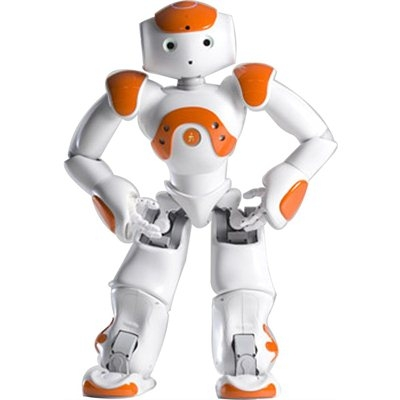
\includegraphics[width=0.35\textwidth]{nao}
\caption{Umanoide NAO.}
\label{fig:ur10}
\end{figure}

\section{Obiettivi e Procedimento}
L'obiettivo di tale esperienza è quello di pianificare il moto di un NAO robot in un ambiente 2D popolato da ostacoli. Il robot dovrà dunque essere comandato per camminare lungo un percorso precalcolato, evitando collisioni con gli ostacoli posti nelle vicinanze. Dunque si dovrà, nell'ordine:
\begin{itemize}
\item Caricare una mappa, utilizzando inizialmente quella predefinita
\item Calcolare il percorso con un software di path planning
\item Far camminare il robot simulato, all'interno dell'ambiente senza collidere
\item Muovere il robot reale, usando la stessa mappa e lo stesso percorso generato nella simulazione.
\end{itemize}
Dopodichè si dovrà caricare una mappa diversa da quella predefinita, e ripetere i punti precedenti. 

\section{Simulazioni}
Attraverso i tool \textit{2D} \textit{Pose} \textit{Estimate} e \textit{2D} \textit{Nav} \textit{Goal} è possibile realizzare la fase di path planning, con la quale verrà calcolato il percorso ottimo, che verrà poi comunicato al NAO, il quale sarà interfacciato con il programma in esecuzione attraverso una rete Ethernet. Per prima cosa, in un ambiente software simulativo, si assegna una posizione di inizio e fine percorso per il NAO, all'interno di una mappa preassegnata comprendente alcuni ostacoli. 


Si procede dunque all'inizializzazione dell'ambiente simulativo con la mappa predefinita, alla quale si va a comunicare la posizione iniziale del robot e quella finale. Come viene visualizzato in Figura \ref{fig:screen1}, il percorso tra posizione iniziale e finale viene calcolato e viene dunque simulato il movimento del robot.
Allo stesso modo, viene caricata una diversa mappa, e ripetuta la simulazione.

\section{Creazione della Mappa}
Per la creazione della mappa si è scritto un semplice programma (\textit{make\_map.cpp}) avviabile con il comando ROS $rosrun \quad esperienza3 \quad make\_map$ una volta installato il pacchetto. Il programma cerca il file \textit{mappa.yaml} all'interno del pacchetto \textit{esperienza 3}, in questo file un qualsiasi utente può specificare:
\begin{itemize}
\item Dimensione della mappa in termini di numero celle in altezza e larghezza.
\item Il numero di ostacoli nella mappa e le loro coordinate $x$ ed $y$.
\item La lunghezza in metri del lato di una singola cella.
\item Il numero di pixel con cui si andrà a disegnare il lato della cella. 
\end{itemize}
Una volta recuperati questi dati crea un'immagine in bianco e nero corrispondente ai dati inseriti nel file \textit{YAML} e la salva all'interno della cartella $maps$ del pacchetto \textit{footstep\_planner} così da poter essere direttamente utilizzata durante l'esperienza prima di terminare l'esecuzione visualizza l'immagine creata. \\
In Figura \ref{fig:tappeto} è rappresentata la mappa restituita dal programma \textit{make\_map} ottenuta con la seguente configurazione, dove i contorni neri e gli assi cartesiani sono stati aggiunti successivamente per rendere la visualizzazione più semplice; essi non sono invece presenti nella mappa che si utilizza per l'esperienza.

\begin{itemize}
\item $altezza = 5$;
\item $lunghezza = 10$;
\item $numero\_ostacoli = 10$;
\item Posizione ostacoli:
	\begin{itemize}
	\item $x = [1,2,2,2,4,4,4,5,6,6]$;
	\item $y = [1,1,2,3,0,2,4,1,2,3]$;
	\end{itemize}
\end{itemize}

\begin{figure}[!h]
\centering
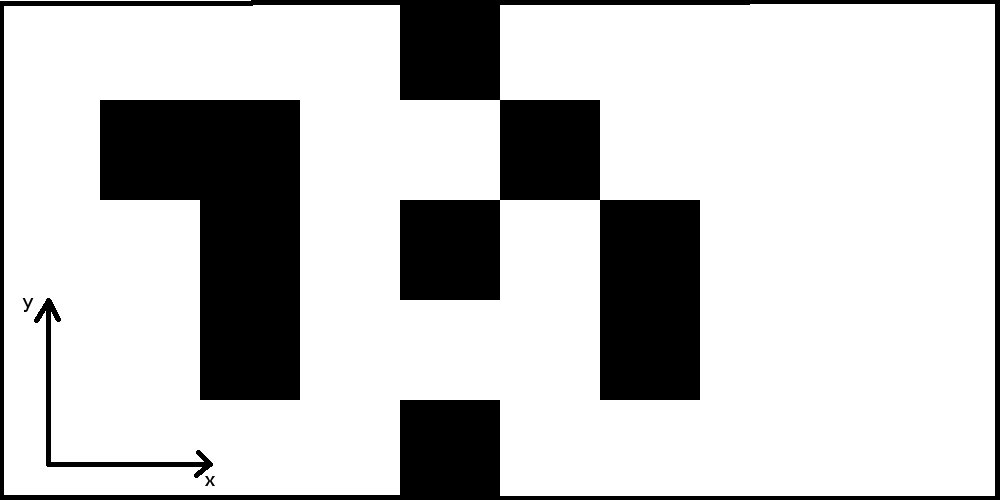
\includegraphics[width=0.6\textwidth]{tappeto}
\caption{Mappa restituita dal programma \textit{make\_map}.}
\label{fig:tappeto}
\end{figure}



\section{Test in laboratorio}
A questo punto è possibile procedere con il test in ambiente reale. Per far collegare il NAO con il programma che eseguirà path planning e movimento del robot è necessario innanzitutto collegare entrambi alla stessa rete LAN. 
Ulteriore passo da fare per far lavorare il NAO nell'ambiente reale, è quello di assicurare che i motori dei giunti siano attivi, in modo che il robot possa inizialmente reggersi in piedi restando fermo. \\
Per prima cosa si procede al calcolo del percorso ottimo su mappa predefinita attraverso l'utility software già menzionata. Dopodichè il percorso calcolato viene comunicato al NAO, che nel frattempo avvia il suo movimento all'interno della mappa predefinita reale, appositamente ricreata, dove si sono posti dei conetti stradali a rappresentazione gli ostacoli (Figura \ref{fig:passo1}).



\begin{figure}[!ht]
\centering
\subfloat[Nella mappa viene mostrato il percorso ottimo, calcolato tra inizio e fine.]	{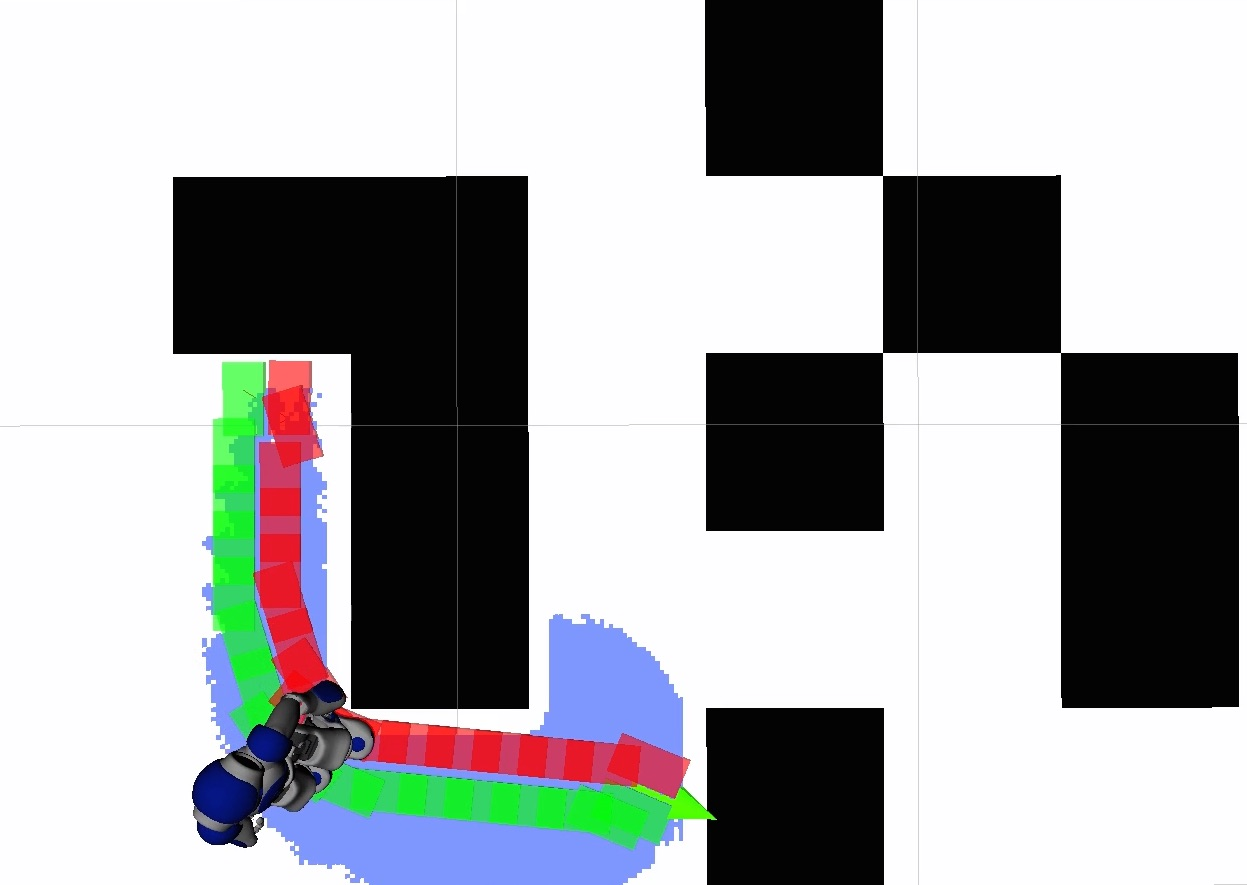
\includegraphics[width=0.5\textwidth]{nao_map}
\label{fig:screen1}}
\subfloat[ Mappa ricreta in ambiente reale, in Laboratorio.]	{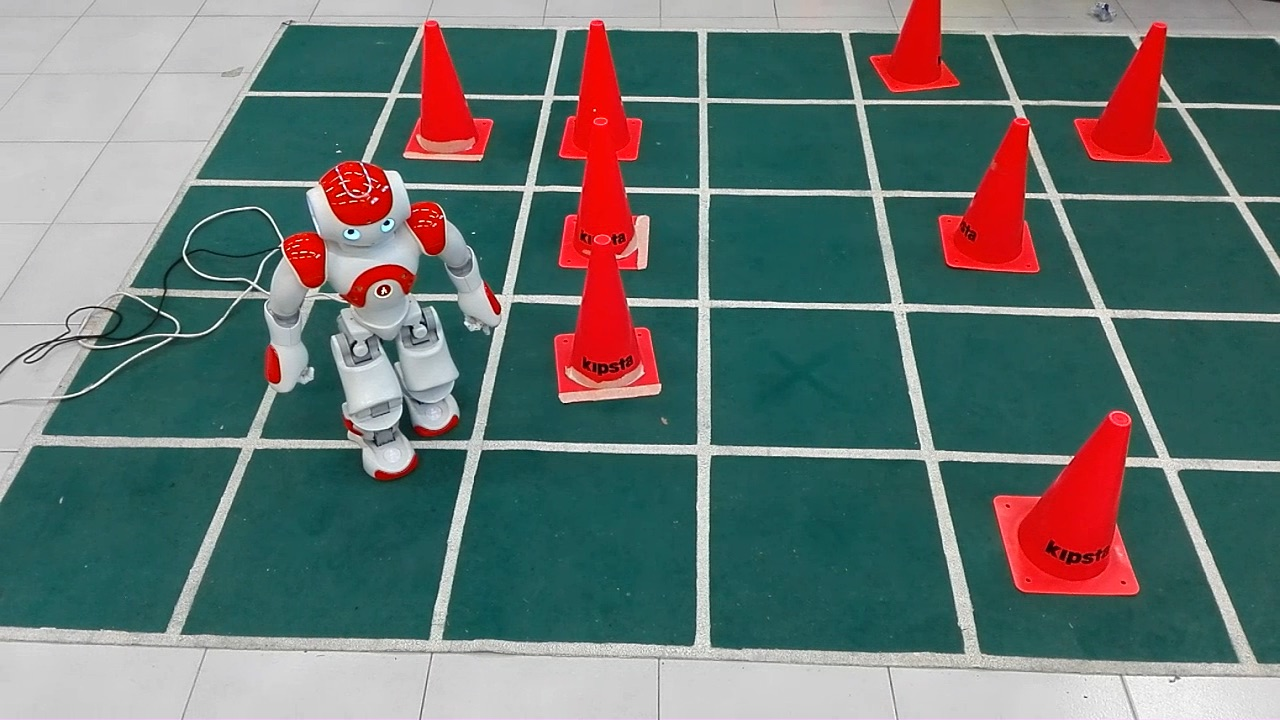
\includegraphics[width=0.5\textwidth]{nao_lab}
\label{fig:passo1}}
\caption{Movimento del Robot.}
%\label{fig: PzPs}
\end{figure}

\newpage

\section{Conclusioni}
Con la presente esperienza si è fatto pratica con i concetti di path planning, obstacle avoiding e con il robot umanoide NAO, con il quale è stato necessario ad esempio risovere il suo interfacciamento con l'host di simulazione, così come problemi iniziali nel mantenere il robot in equilibrio nella sua posizione iniziale. Le simulazioni del robot su software non hanno riscontrato particolari problematiche, mentre i test sul robot reale hanno evidenziato ricorrenti problemi nel seguire le traiettorie prepianificate, principalmente per il fatto che un continuo stress dei motori, portava questi ultimi ad un eccessivo surriscaldamento. Per far fronte a questo problema si è preferito scegliere una traiettoria che non fosse troppo lunga in modo da non sollecitare eccessivamente il robot. Dopo ciò anche i test in ambiente reale hanno conferito risultati soddisfacenti.



\clearpage

\end{document}